% Revisión documental de Fase 3: 31-10-2026.
\section{Arquitectura general del sistema}
\label{sec:arq}
\subsection{Alcance y fuente de verdad}
Esta revisión toma como fuente principal el código local de
\nolinkurl{EventoCultural_Integrado/EventoCultural_Integrado}. La rama de referencia
es \url{https://github.com/sunsitox/Proyecto_Capston_Evento_Cultural/tree/deploy/vercel-preview}.
No se certifica igualdad entre la copia local y esa rama ni que todas las funciones
locales estén desplegadas. Se distingue implementación, configuración remota y
verificación de extremo a extremo.

\begin{itemize}[leftmargin=1.4em]
\item \textbf{Recolección:} scraper Python independiente, con conectores, saneamiento,
NVIDIA NIM selectivo y checkpoints SQLite. Su evidencia operativa conservada corresponde
al ciclo del 11-10-2026; no constituye una nueva ejecución del scraper.
\item \textbf{Persistencia:} Supabase/PostgreSQL, catálogo y perfiles con políticas RLS;
Supabase Auth para sesiones y Storage para avatares.
\item \textbf{Cliente:} SPA Angular 22 e Ionic 9, con servicios TypeScript y signals.
Consulta catálogo y autenticación mediante \texttt{@supabase/supabase-js}.
El código Python de \texttt{backend/} es legado y no es una dependencia del flujo web actual.
\item \textbf{Servidor:} Supabase Edge Functions para operaciones privilegiadas:
\texttt{registrar-cuenta}, \texttt{admin-account}, \texttt{publicar-evento},
\texttt{admin-eventos}, \texttt{reset-password-request},
\texttt{reset-password-confirm} y \texttt{recomendaciones-semanal}.
La clave de servicio pertenece exclusivamente al servidor.
\item \textbf{Entrega:} Vercel para la SPA, GitHub Actions para el scraper y Capacitor
para Android. No se utiliza Docker en la estrategia adoptada.
\end{itemize}

\begin{figure}[H]\centering
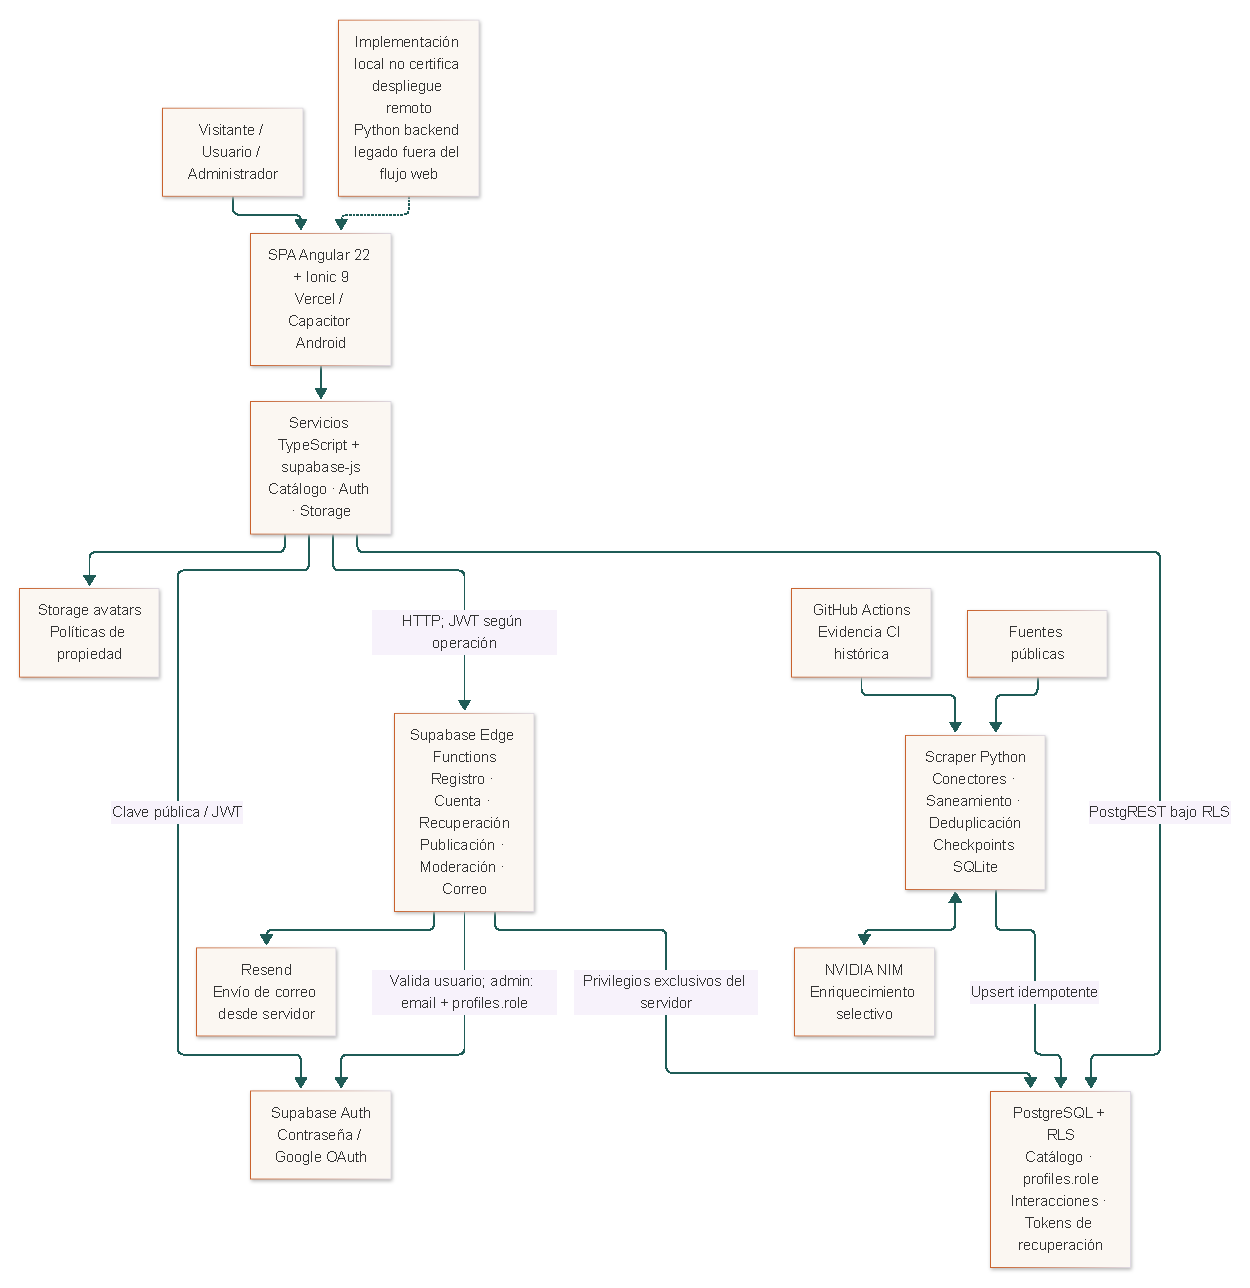
\includegraphics[width=\textwidth,height=0.70\textheight,keepaspectratio]{01_arquitectura_general.pdf}
\caption{Arquitectura actual; fuente editable: Diagramas/01\_arquitectura\_general.mmd.}
\label{fig:arq}\end{figure}

\subsection{Contratos y límites de confianza}
\begin{longtable}{p{3.1cm}p{4.0cm}p{7.0cm}}
\toprule Origen y destino & Contrato & Regla de acceso \\\midrule\endhead
Cliente a Supabase & Catálogo mediante PostgREST; sesión mediante Auth & Clave pública y JWT del usuario; las políticas RLS gobiernan los datos. \\
Registro a función Edge & Correo, contraseña y nombre & Crea cuenta confirmada mediante Admin API; luego el cliente inicia sesión. No comprueba la propiedad del buzón. \\
Usuario a publicar-evento & Datos validados del evento y JWT & Identidad obtenida con getUser; crea evento draft y no acepta status/source\_id del cliente. \\
Administrador a admin-eventos & Listado y acciones de moderación & Valida JWT, proveedor email y profiles.role=admin antes de utilizar privilegios de servicio. \\
Recuperación a funciones Edge & Solicitud por correo y confirmación con token & JWT firmado y registro password\_reset\_tokens con caducidad y marca de uso; requiere migración y secretos. \\
Servidor a correo & API de Resend & Clave privada en el entorno de funciones. Envío implementado no equivale a recepción demostrada. \\
\bottomrule\end{longtable}

\section{Arquitectura del scraper}
\label{sec:scraper}
El pipeline carga fuentes declarativas, selecciona conectores por Strategy/Factory,
sanea y deduplica eventos, normaliza ubicaciones, exporta JSON/CSV y sincroniza
Supabase por upsert. Los checkpoints SQLite permiten reanudar trabajo y reutilizar
resultados de IA de eventos sin cambios. El límite configurado de NVIDIA es 40 RPM;
no se presenta como una garantía contractual del proveedor.

\begin{figure}[H]\centering
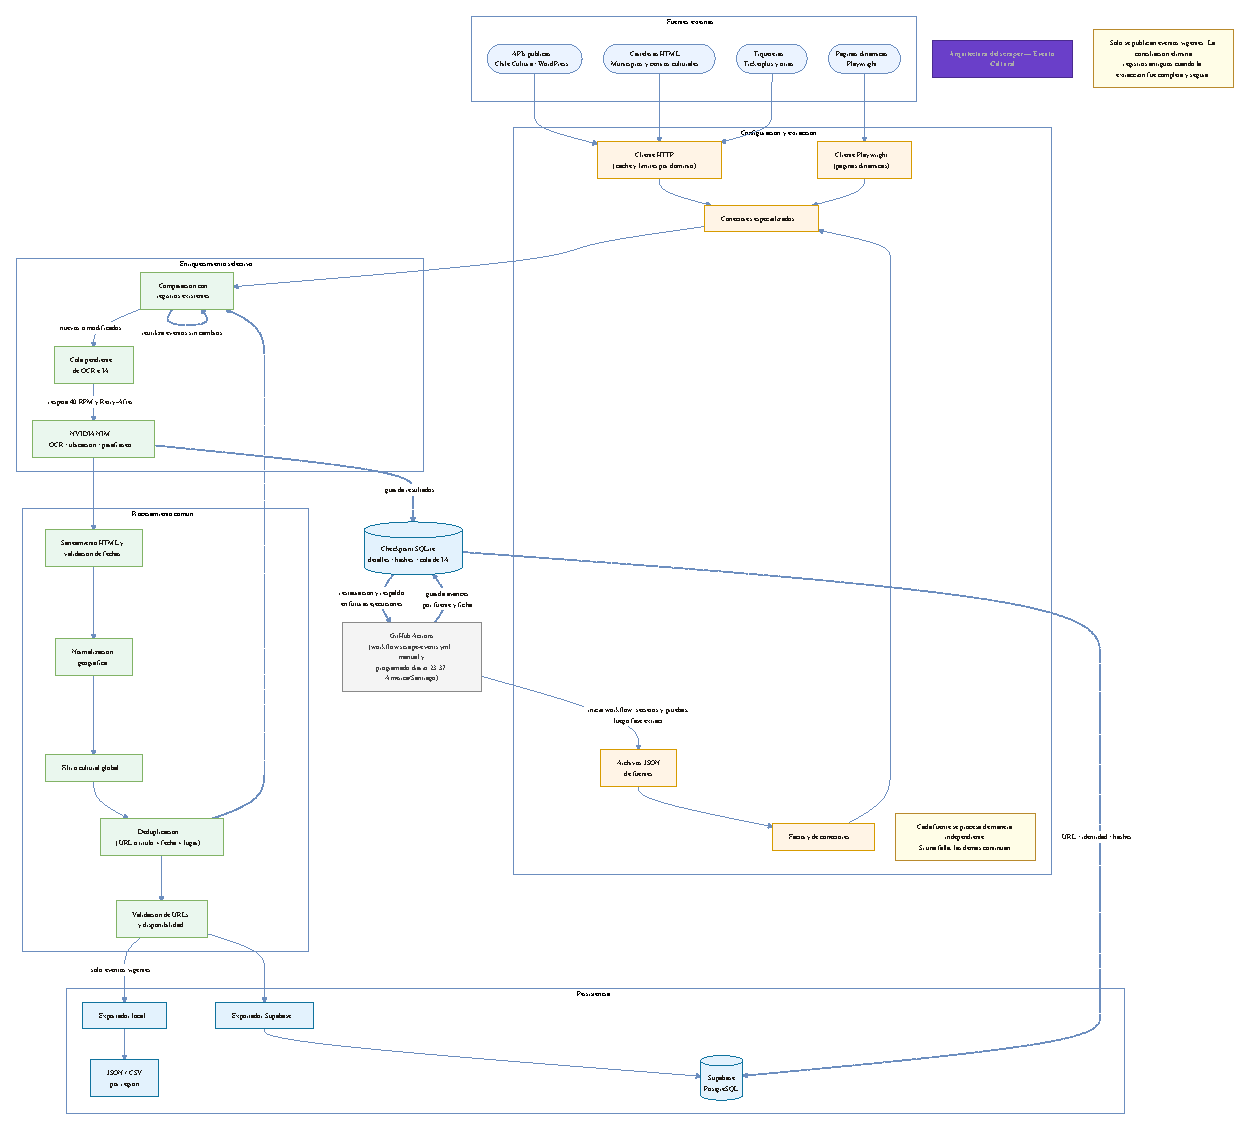
\includegraphics[width=0.94\textwidth]{07_arquitectura_scraper.pdf}
\caption{Pipeline del scraper conservado de la línea base; verificar su inventario vigente antes del cierre.}
\label{fig:scraper-arq}\end{figure}

El inventario de 21 fuentes permanentes y una estacional y las ejecuciones de CI
corresponden a evidencia histórica. No se infiere que todas sigan disponibles hoy.
Los conectores aíslan fallos por fuente; la conciliación y el borrado de vencidos
dependen de la configuración y de una extracción completa. GitHub Actions no garantiza
puntualidad: el desfase del run 25 sigue registrado como DEF-CI-001.

\section{Arquitectura del frontend}
\label{sec:frontend}
\subsection{Stack y organización}
Según \texttt{package.json}: Angular 22.0.1, Ionic 9, TypeScript 6,
Capacitor 8, supabase-js 2, Leaflet 1.9.4, RxJS 7.8 y Vitest 4 con jsdom.
\texttt{core/} concentra modelos y servicios; \texttt{pages/} las pantallas;
\texttt{features/home/} los layouts; y \texttt{layout/} la navegación adaptativa.
Las versiones resueltas deben reproducirse con \texttt{package-lock.json}.

\begin{figure}[H]\centering
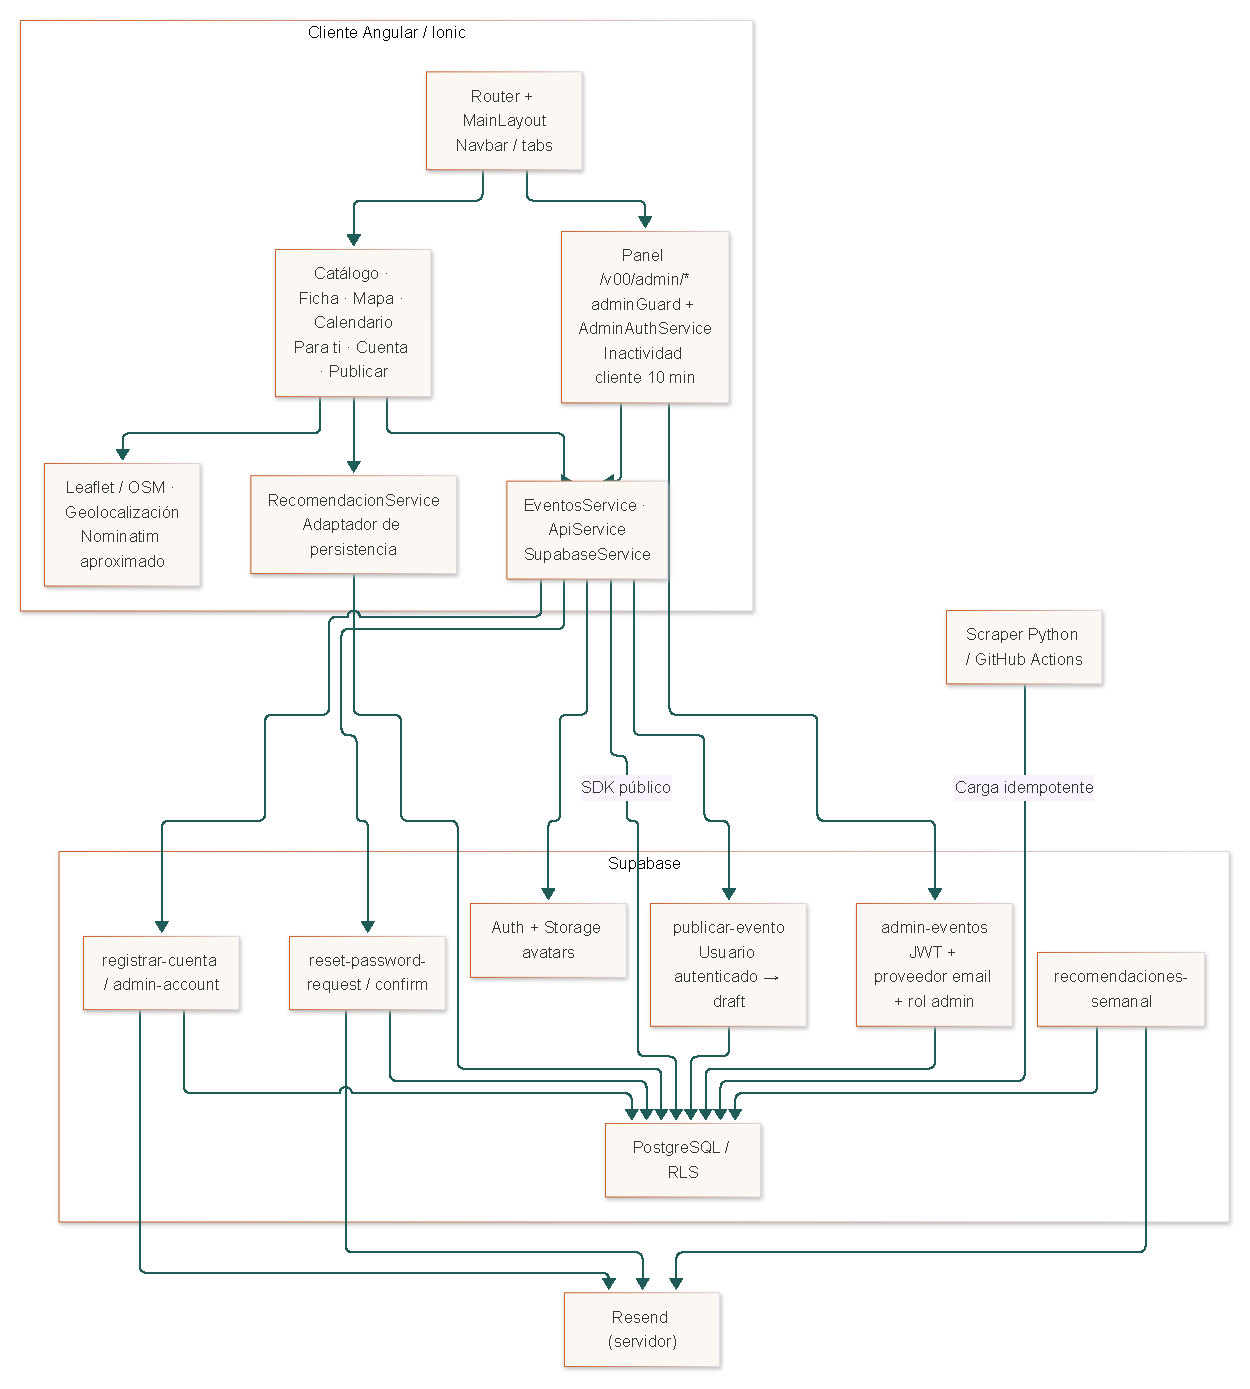
\includegraphics[width=0.95\textwidth,height=0.68\textheight,keepaspectratio]{02_componentes.pdf}
\caption{Componentes actuales y separación cliente/servidor.}
\label{fig:comp}\end{figure}

\subsection{Descubrimiento y personalización}
El catálogo publicado alimenta búsqueda, filtros combinados, detalle, calendario y
mapa Leaflet/OpenStreetMap. Nominatim aporta geocodificación de respaldo con cola,
caché y límites; los resultados aproximados no sustituyen coordenadas verificadas.
La geolocalización usa Capacitor en Android y alternativa web.
Las recomendaciones se calculan por señales de interés, no por un modelo generativo:
\texttt{RecomendacionService} calcula afinidad y razones; el adaptador de persistencia
almacena interacciones en \texttt{user\_event\_interactions} y preferencias en metadata.
Los invitados mantienen estado en memoria. El respaldo de eventos de demostración no
debe confundirse con una consulta remota exitosa.

\subsection{Cuenta y perfil}
El registro principal llama \texttt{registrar-cuenta}, que crea el usuario con
\texttt{email\_confirm=true}; el cliente ejecuta \texttt{signInWithPassword} sin
exigir verificación del buzón. La función intenta enviar un correo de registro exitoso
por Resend. Existe respaldo legacy con \texttt{signUp}: si la función no está disponible,
puede reaparecer la confirmación de Supabase. Por tanto, la experiencia solicitada
requiere desplegar y configurar la función, no solo cambiar el formulario.

El perfil permite editar nombre, contraseña e imagen. Storage utiliza el bucket
\texttt{avatars}; el metadata \texttt{avatar\_url\_custom} tiene prioridad sobre la imagen
OAuth, y esta se utiliza si no hay imagen propia. La identidad reactiva alimenta perfil
y navegación. Google OAuth tiene botón y callback implementados; su configuración remota
y la recepción de correos no se certifican por inspección de código.
La recuperación actual usa las funciones \texttt{reset-password-request/confirm} y
\texttt{/restablecer-contrasena?token=...}, no únicamente el flujo antiguo de GoTrue.

\subsection{Administración y publicación}
Las rutas \texttt{/v00/admin/*} requieren \texttt{adminGuard}; no enlazarlas públicamente
no constituye una medida de autorización. \texttt{AdminAuthService} consulta
\texttt{profiles.role} y solo admite \texttt{admin}, con proveedor email: visitor,
editor y Google son rechazados. El rol editable de metadata no es autoridad administrativa.
La función \texttt{admin-eventos} repite las comprobaciones en el servidor.
El cliente cierra la sesión tras 10 minutos sin interacción, comprobados cada 15 segundos,
y redirige al ingreso con aviso. La última actividad se reinicia al recargar; no es un
timeout absoluto persistido ni una revocación impuesta por el servidor.

La publicación autenticada crea un borrador mediante \texttt{publicar-evento};
\texttt{admin-eventos} implementa listado administrativo, publicación y supresión.
El dashboard calcula métricas del catálogo cargado en el cliente: no equivale a analítica
comercial ni a estadísticas certificadas de uso. La ocultación de fuentes en el navegador
no equivale a detener el scraper ni a persistir una decisión global.

\subsection{Despliegue y pendientes}
\texttt{angular.json} genera \texttt{www}; \texttt{vercel.json} ya incluye la reescritura
SPA a \texttt{/index.html}. Existe proyecto Android y APK debug local; esto no demuestra
instalación, GPS u OAuth en dispositivo físico ni publicación en tienda.
Quedan por registrar: regresión del ciclo QA histórico, pruebas remotas de autorización,
correo y recuperación, aislamiento entre usuarios, pruebas nativas y mediciones de
rendimiento/accesibilidad. Ninguno de esos resultados se deduce de una compilación.
